\documentclass[11pt,a4paper]{article}\usepackage[]{graphicx}\usepackage[]{color}
% maxwidth is the original width if it is less than linewidth
% otherwise use linewidth (to make sure the graphics do not exceed the margin)
\makeatletter
\def\maxwidth{ %
  \ifdim\Gin@nat@width>\linewidth
    \linewidth
  \else
    \Gin@nat@width
  \fi
}
\makeatother

\definecolor{fgcolor}{rgb}{0.345, 0.345, 0.345}
\newcommand{\hlnum}[1]{\textcolor[rgb]{0.686,0.059,0.569}{#1}}%
\newcommand{\hlstr}[1]{\textcolor[rgb]{0.192,0.494,0.8}{#1}}%
\newcommand{\hlcom}[1]{\textcolor[rgb]{0.678,0.584,0.686}{\textit{#1}}}%
\newcommand{\hlopt}[1]{\textcolor[rgb]{0,0,0}{#1}}%
\newcommand{\hlstd}[1]{\textcolor[rgb]{0.345,0.345,0.345}{#1}}%
\newcommand{\hlkwa}[1]{\textcolor[rgb]{0.161,0.373,0.58}{\textbf{#1}}}%
\newcommand{\hlkwb}[1]{\textcolor[rgb]{0.69,0.353,0.396}{#1}}%
\newcommand{\hlkwc}[1]{\textcolor[rgb]{0.333,0.667,0.333}{#1}}%
\newcommand{\hlkwd}[1]{\textcolor[rgb]{0.737,0.353,0.396}{\textbf{#1}}}%
\let\hlipl\hlkwb

\usepackage{framed}
\makeatletter
\newenvironment{kframe}{%
 \def\at@end@of@kframe{}%
 \ifinner\ifhmode%
  \def\at@end@of@kframe{\end{minipage}}%
  \begin{minipage}{\columnwidth}%
 \fi\fi%
 \def\FrameCommand##1{\hskip\@totalleftmargin \hskip-\fboxsep
 \colorbox{shadecolor}{##1}\hskip-\fboxsep
     % There is no \\@totalrightmargin, so:
     \hskip-\linewidth \hskip-\@totalleftmargin \hskip\columnwidth}%
 \MakeFramed {\advance\hsize-\width
   \@totalleftmargin\z@ \linewidth\hsize
   \@setminipage}}%
 {\par\unskip\endMakeFramed%
 \at@end@of@kframe}
\makeatother

\definecolor{shadecolor}{rgb}{.97, .97, .97}
\definecolor{messagecolor}{rgb}{0, 0, 0}
\definecolor{warningcolor}{rgb}{1, 0, 1}
\definecolor{errorcolor}{rgb}{1, 0, 0}
\newenvironment{knitrout}{}{} % an empty environment to be redefined in TeX

\usepackage{alltt}
\usepackage[top=1.00in, bottom=1.0in, left=1.1in, right=1.1in]{geometry}
\usepackage{graphicx}
\usepackage[numbers]{natbib}
\bibliographystyle{..//bib/styles/nature.bst}

\usepackage[export]{adjustbox}
\IfFileExists{upquote.sty}{\usepackage{upquote}}{}
\begin{document}

\noindent 2011 Crystal Dr \#600\\
\noindent Arlington, VA, 22202\\

\vspace{1.5ex}

\pagenumbering{gobble}

\noindent{Dear Dr. Wagner-Riddle:}  
\vspace{3ex}\\
\noindent Please consider our manuscript entitled `Variation across space, species and methods in models of spring phenology' as a Research Paper for \textit{Agricultural and Forest Meteorology}. \\

\noindent As climate change and urbanization increase, predicting spring plant phenology in temperate forests is critical for forecasting important processes such as carbon storage. The growing degree day (GDD) model is a major forecasting method, but required GDD is predicted to shift with changes in climate, especially warmer winters. Here we combine simulations and new observations with Bayesian hierarchical models to assess how consistent GDD models of budburst are across species and landscapes. We assessed the effects of an urban arboretum versus a more rural forested site coupled with the effect of climate data type (i.e., weather station versus HOBO logger temperature data) across 17 species. We also present an interactive Shiny application that aims to enhance understanding of our results and aid future studies. \\

\noindent We found that estimated GDD thresholds can vary over 200\% across species and up to 20\% across sites and methods. Our results showed the urban site was warmer (by almost 3 $\degree$C in the spring), but this did not translate to individuals requiring more GDDs as we hypothesized, but rather fewer GDDs until budburst. Further, we found a strong microclimate effect apparent by the large variation in GDD with method. Our results suggest that forecasts based on GDD models for spring phenology have inherent accuracy issues, and estimates vary strongly across space, species and warming. Our research improves our understanding of GDD models and suggests ways to refine models of spring phenology and, in turn, improve forecasts for temperate forests. \\

\noindent Both authors substantially contributed to this work and approved of this version for submission. The manuscript is 4680 words, with a 278 word summary and five figures. We hope that you will find it suitable for publication in \textit{Agricultural and Forest Meteorology}. Thank you for your consideration. \\

\vspace{1.5ex}
\noindent Sincerely, \\
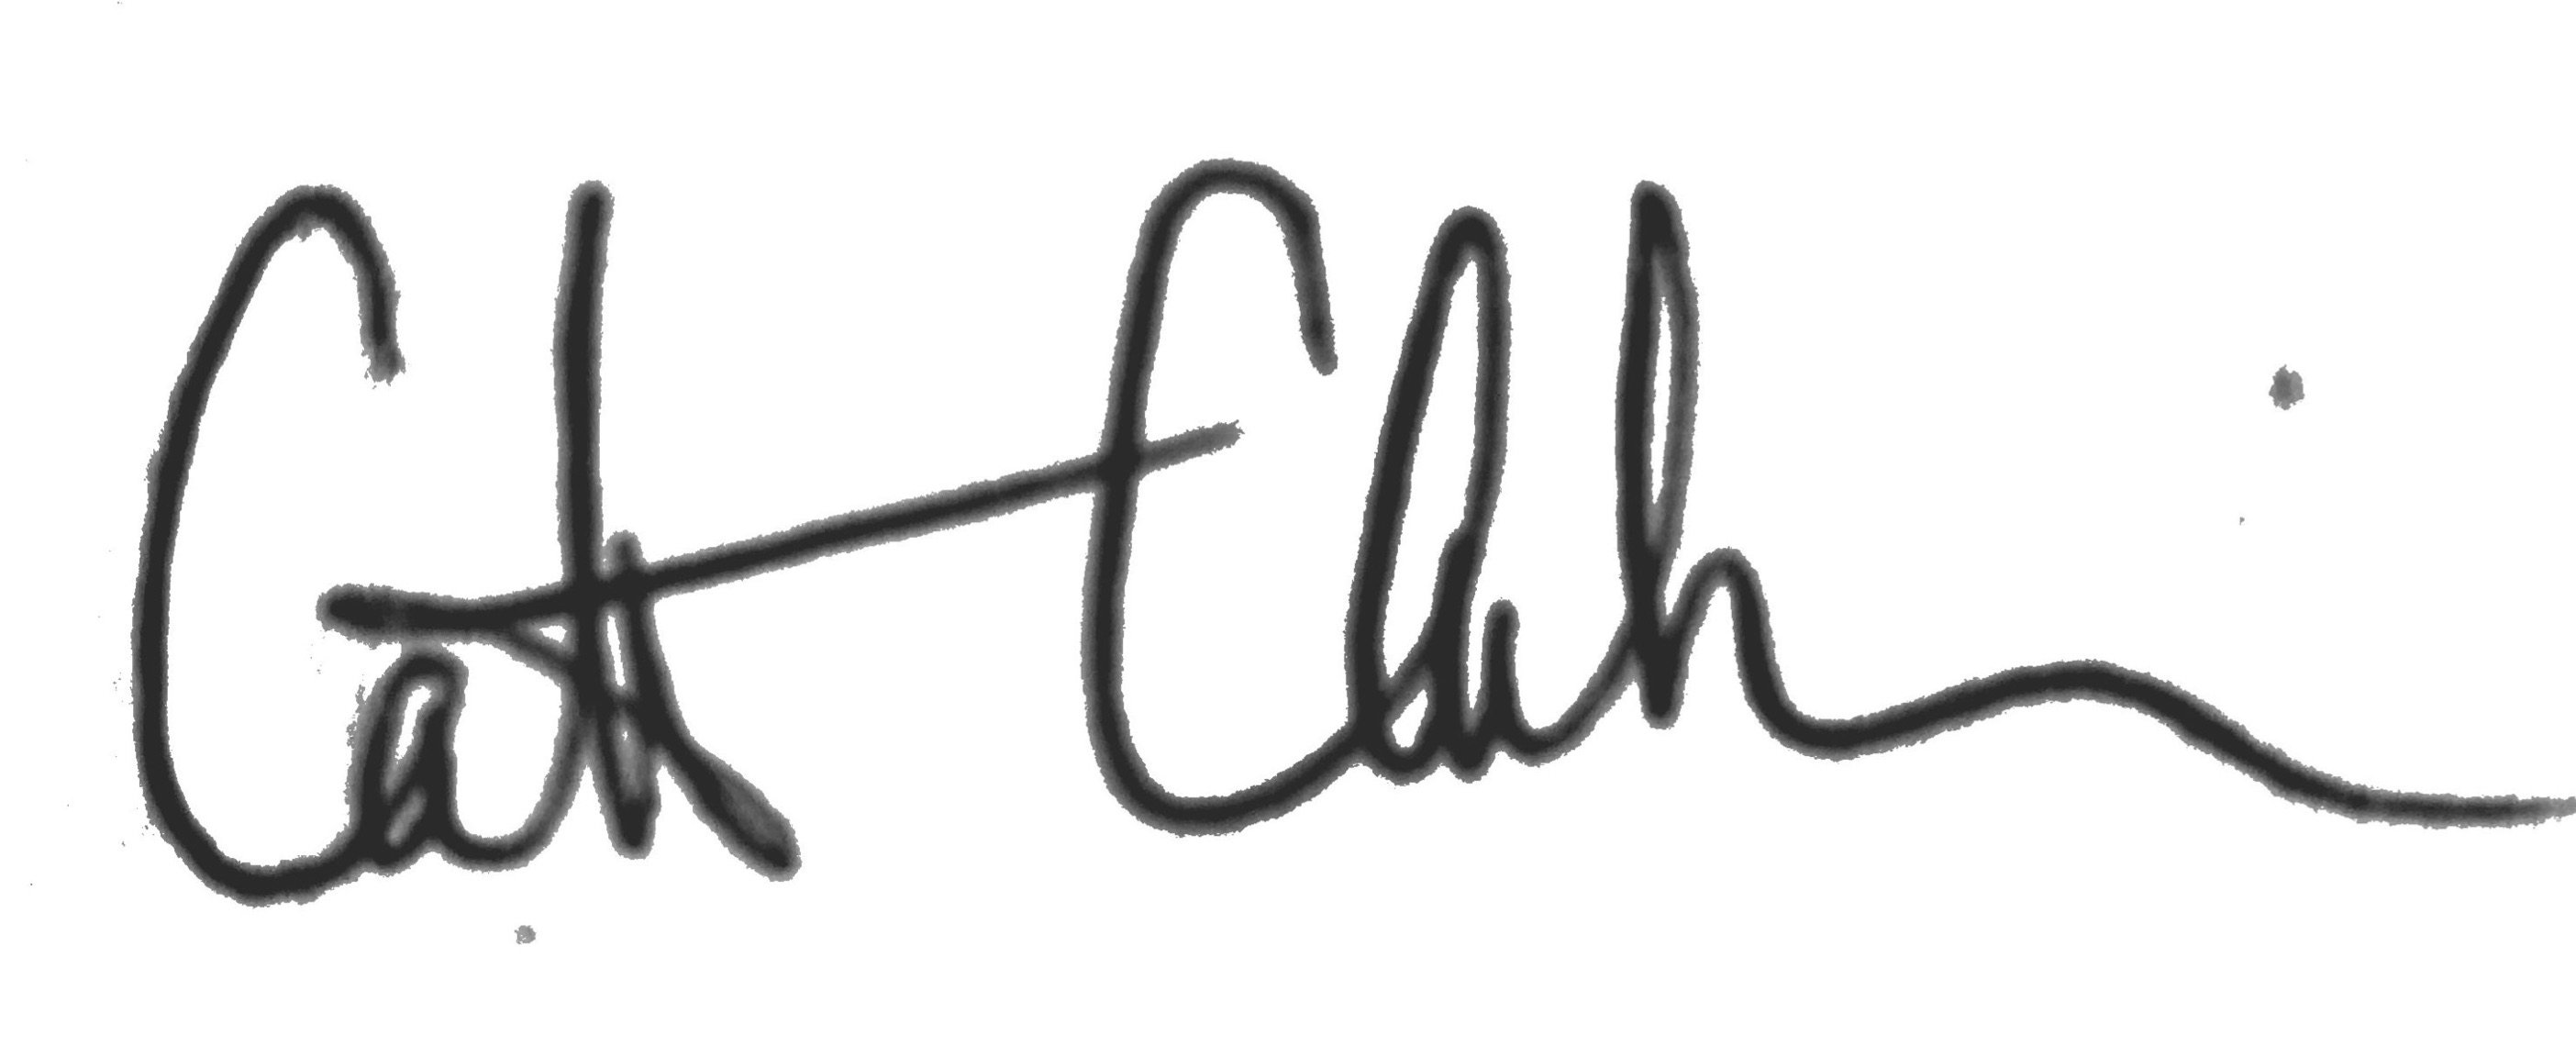
\includegraphics[width=0.2\textwidth]{full_signature.jpg} \\
\noindent Catherine Chamberlain (on behalf of my co-author)
\vspace{2ex}\\
\noindent Authors:\\
C. J. Chamberlain $^{1,2,3}$ \& E. M. Wolkovich $^{1,2,4}$
\vspace{2ex}\\
\emph{Author affiliations:}\\
$^{1}$Arnold Arboretum of Harvard University, 1300 Centre Street, Boston, Massachusetts, USA; \\
$^{2}$Organismic \& Evolutionary Biology, Harvard University, 26 Oxford Street, Cambridge, Massachusetts, USA; \\
$^{3}$Conservation International, Arlington, VA, USA;\\
$^{4}$Forest \& Conservation Sciences, Faculty of Forestry, University of British Columbia, 2424 Main Mall, Vancouver, BC V6T 1Z4;\\
\vspace{2ex}
$^*$Corresponding author: 248.953.0189; cchamberlain@conservation.org

\end{document}
